\section{Auswertung}
\label{sec:auswertung}
In diesem Kapitel werden die aufgenommenen Messwerte ausgewertet.
\subsection{Zählrohr Charakterristik}
\label{sec:characteristik}
In diesem Abschnitt wird die sogenannte Charakeristik des Geiger-Müller-Zählrohres ermittelt. Dazu wird der
Abstand der Strahlungsquelle so gewählt, das die Impulsrate bei etwa $10000 Imp/min$ liegt um eine zu große 
Ungenauigkeit durch Totzeiten zu vermeiden. Da die Messwerte poissonverteilt sind wird der Fehler über \autoref{eq:poisson}
\begin{figure}
    \centering
    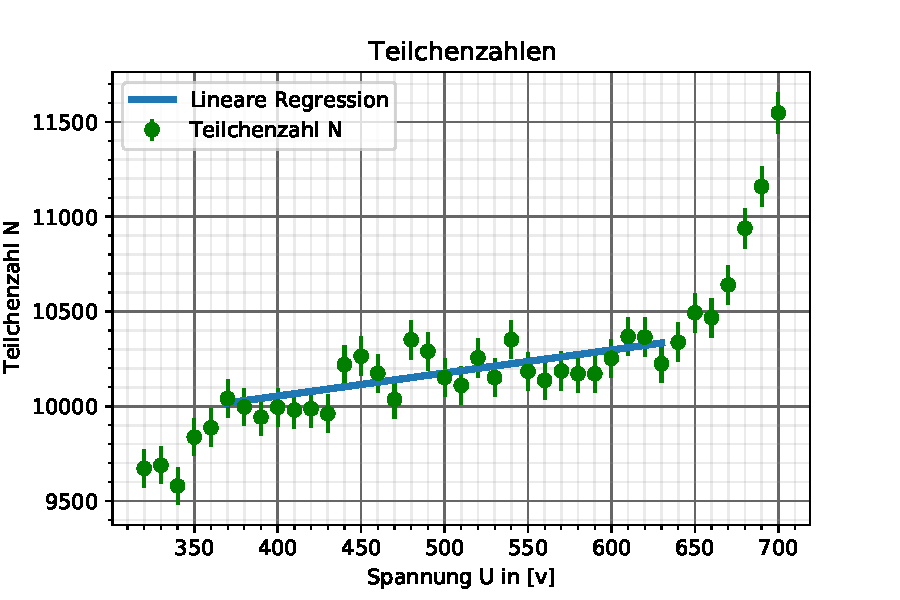
\includegraphics{kennlinie.pdf}
    \caption{Teilchenzahlen im Geiger-Müller-Zählrohr}
    \label{fig:teilchenzahl}
  \end{figure}
Um die Plateau-Steigung zu ermittlen wurde mittels linearer Regression ein Polynom ersten Grades der 
Form $f(x)=ax+b$ durch die Messpunkte gelegt:
\begin{center}
    $f(x)=(1.215\pm0.256)x + (9567.924\pm125.414)$ $\rightarrow$ $D_f=\{x\in\mathbb{R} \vert 360\le x\le620\}$    
\end{center}
Das Plateau hat eine Länge von etwa $\SI{260}{V}$ im Bereich von $\SI{360}{V}$ bis $\SI{620}{V}$ und  eine 
Steigung von $\SI{1,215\pm0,256}{\frac{\%}{100}}$.
\subsection{Totzeit des Zählrohres}
\label{sec:totzeit}
An dieser Stelle wird zunächst mithilfe eines Oszilloskopes die Totzeit des Geiger-Müller-Zählrohres
abgeschätzt und anschließend mit der Zwei-Quellen-Methode genauer vermessen bzw. abgeschätzt. 
\subsubsection{Totzeitbestimmung mit dem Oszilloskop}
\label{sec:totzeitO}
In \autoref{fig:oszilloskop} ist die Bildröhre eines Oszilloskopes zu sehen. Die Totzeit ist der Raum 
zwischen den ersten beiden Signalen. Da das Oszilloskop auf 100µs/DIV eingestellt ist und die beiden Signale 
innerhalb einer Unterteilung der DIV liegen muss die Totzeit $T<20µs$ sein. Da der Signalabstand sehr klein ist 
wird die Totzeit auf $T \approx 2µs$ geschätzt.
\begin{figure}
  \centering
  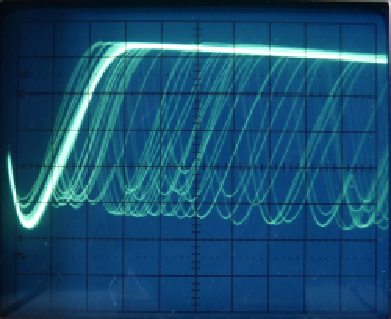
\includegraphics{oszilloskop.pdf}
  \caption{Signal am Geiger-Müller-Zählrohr 100µs/DIV}
  \label{fig:oszilloskop}
\end{figure}
\subsubsection{Totzeitbestimmung mit der Zwei-Quellen-Methode}
\label{sec:totzeitZ}
Die Totzeit lässt sich mit der Näherungsformel \autoref{eq:totzeit} aus den Messwerten 
\autoref{sec:werteTotzeit} für $N_1$, $N_2$ und $N_{1+2}$ sofort ermittlen, es folgt also:
\begin{center}
  $T=(0.96\pm0.04) µs$
\end{center}
Der entsprechende Fehler wurde mit der Gaußschen-Fehlerfortpflanzung \autoref{eq:gaussfehler} ermittelt.
Dazu wurden folgende Ableitungen verwendet:
\begin{center}
  $\frac{\partial T}{\partial N_1}=\dfrac{c-b}{2ba^2}$\\
\end{center}
\begin{center}
  $\frac{\partial T}{\partial N_2}=\dfrac{c-a}{2ab^2}$\\
\end{center}
\begin{center}
  $\frac{\partial T}{\partial N_{1+2}}=-\dfrac{1}{2ab}$
\end{center}

\subsection{Ladung pro einfallendem Teilchen}
\label{sec:ladung}
Im folgenden Diagramm \autoref{fig:ladungProTeilchen} ist die Anzahl der Ladungen $Z$ die durch ein einziges einfallendes Teilchen ausgelöst
wurden gegen die Spannung aufgetragen. Die Zahl $Z$ lässt sich mit den Werten aus \autoref{sec:werteStrom} 
direkt über \autoref{eq:zaehlrohrstrom} berechnen
\begin{figure}
  \centering
  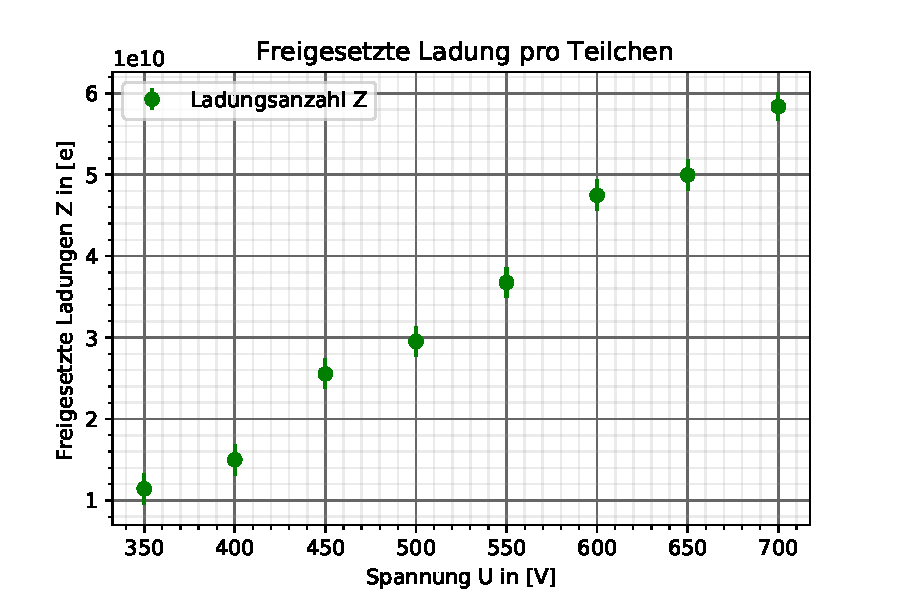
\includegraphics{ladungproteilchen.pdf}
  \caption{Pro einfallendem Teilchen ausgelöste Ladung}
  \label{fig:ladungProTeilchen}
\end{figure}
